\begin{figure}[tbp]
\centering
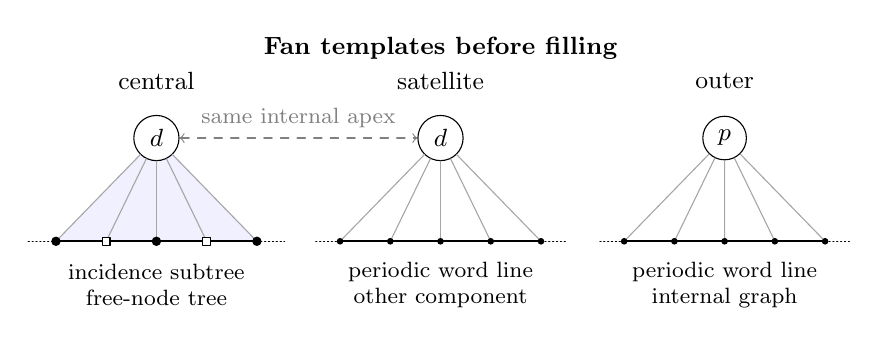
\begin{tikzpicture}[x=.88cm,y=.88cm,font=\small,
  every node/.style={align=center},line cap=round,line join=round,
  apex/.style={circle,draw,fill=white,inner sep=3pt},
  slot/.style={rectangle,draw,fill=white,inner sep=2pt}]
  \node[font=\small\bfseries] at (6,6.22)
    {Fan templates before filling};
  \node at (1.9,5.75) {central};
  \node at (6,5.75) {satellite};
  \node at (10.1,5.75) {outer};
  \fill[blue!6] (.45,3.43)--(1.9,4.92)--(3.35,3.43)--cycle;
  \node[apex] (dc) at (1.9,4.92) {$d$};
  \node[apex] (ds) at (6,4.92) {$d$};
  \node[apex] (po) at (10.1,4.92) {$p$};
  \draw[<->,dashed,gray] (dc)--node[above,font=\footnotesize]
    {same internal apex} (ds);
  \foreach \x in {.45,1.175,1.9,2.625,3.35} {
    \draw[gray!70] (dc)--(\x,3.43);
  }
  \draw[thick] (.45,3.43)--(3.35,3.43);
  \foreach \x in {.45,1.9,3.35} {\fill (\x,3.43) circle (1.7pt);}
  \foreach \x in {1.175,2.625} {
    \draw[fill=white] (\x-.055,3.375) rectangle (\x+.055,3.485);
  }
  \draw[densely dotted] (.05,3.43)--(.45,3.43);
  \draw[densely dotted] (3.35,3.43)--(3.75,3.43);
  \foreach \offset/\tip in {4.55/ds,8.65/po} {
    \draw[thick] (\offset,3.43)--(\offset+2.9,3.43);
    \draw[densely dotted] (\offset-.35,3.43)--(\offset,3.43);
    \draw[densely dotted] (\offset+2.9,3.43)--(\offset+3.25,3.43);
    \foreach \step in {0,.725,1.45,2.175,2.9} {
      \draw[gray!70] (\tip)--(\offset+\step,3.43);
      \fill (\offset+\step,3.43) circle (1.2pt);
    }
  }
  \node[font=\footnotesize,text width=3cm] at (1.9,2.8)
    {incidence subtree\\free-node tree};
  \node[font=\footnotesize,text width=3cm] at (6,2.8)
    {periodic word line\\other component};
  \node[font=\footnotesize,text width=3cm] at (10.1,2.8)
    {periodic word line\\internal graph};
\end{tikzpicture}
\caption{The three fan types before filling. The two $d$-symbols are
separate templates for one physical internal apex. Central fans cone
incidence subtrees in free-node Cayley trees; dots are ordinary sites and
small squares are horizontal midpoints. Satellite fans cone indexed word
lines mapping into other central components. Distinct satellite arms at
$d$ target distinct components in the developed model. An outer fan has
its own apex $p$ and an indexed word line mapping into the internal graph.
The word-line maps may repeat physical vertices and edges; their tags
retain the occurrences. The drawings are schematic and impose no planar
geometry.}
\label{fig:fan-templates}
\end{figure}
